\documentclass[12pt, letterpaper, twoside]{article}
\usepackage[utf8]{inputenc}

%set up color scheme
\usepackage{xcolor}
\usepackage{sectsty}
\sectionfont{\color{blue}}  
\subsectionfont{\color{cyan}}  

%package for imbedding images and math
\usepackage{graphicx}
\usepackage{amsmath}

%define the information in the title
\title{\color{cyan}IKEcoin: \\ 
\large A decentralized token economy empowering humans with controlling ownership of their social media data}
\author{Claire Longo, Isaac Longo}
\date{June 2021}

\begin{document}

\maketitle

%insert IKEcoin art
\begin{figure}[h]
  
\includegraphics[scale=0.3]{media/IKEcoin.jpg}
  \centering
\end{figure}

\begin{abstract}
\textit{IKEcoin-Auth is a social sign-on protocol that allows individual consumers to trade their data for personal profit using an Ethereum based assets token IKEcoin. This whitepaper describes this new data marketplace, gives an overview of the system design and token economy, and lays out a roadmap for creating the first version of the IKEcoin system }
\end{abstract}
 \pagebreak

\section{Motivation}
The purpose of this project is to disrupt the data market by giving individual consumers controlling ownership over their own personal social media data. Data is commonly referred to as the new oil because it is one of the most valuable assets in today's economy. Organizations use data to drive decision making, automate complex processes, and curate personalized experiences for their customers. Although companies view this data as hugely valuable asset to drive their business, individual consumers are not directly compensated when their personal data is collected or used. \\

Humans should own their own data as a personal asset. They should be given the choice to either sell it for profit, or keep it private. The marketplace for these data transactions should be clear and easy to use so all humans can fairly engage in the data market. \\

The IKEcoin-Auth is a social login method that allows users to log into websites with a single username and password. This single login authorizes organizations to access the user's data from all social media accounts the user has linked to their IKEcoin. That accessed through IKEcoin-Auth is paid for in IKEcoin tokens, an asset token built on ETH blockchain. This system creates a new marketplace where data is the gold-standard for the value of the IKEcoin tokens traded. \\

\section{System Design}
Coming soon...


\section{Token Economics}
IKEcoin is a soft asset Ethereum token for data transactions through IKEcoin-Auth; a social login protocol for selling personal data. Soft asset tokens are backed by the value of a real asset that is not physical or tangible. In this case IKEcoin is backed by data as the soft asset. The token offers a secure and scalable way to buy and sell data and allow the decentralized economy to place a fair price on the data asset itself. \\

IKEcoin tokens can be traded on the cryptocurrency market, allowing the crypto market to set the price of the social media data in IKEcoin. IKEcoin users earn tokens by connecting social accounts and selling this data to interested parties by their IKEcoin-Auth login protocol to log into websites. Customers pay the users in IKEcoin tokens when the user logs into their website with IKEcoin-Auth protocol. At any time, IKEcoin tokens can be converted to other coins, tokens, or cash. \\

The price paid to the user is based on the market value for social data and the volume and quality of data the user has connected to their IKEcoin-Auth protocol. Let \\
\begin{quote}
$M =$ the fair market value for one unit of data\\
$X =$ the size of the user's data\\
$s =$ the number of social media accounts the user has connected\\
$S =$ the total number of social accounts supported\\
\end{quote}
The price the customer is requested to pay to the user through an IKEcoin-Auth transaction is \\
\begin{equation} 
price=\frac{s}{S} \times M \times x 
\end{equation}

For every IKEcoin transaction, the price of the data is recorded on the Ethereum blockchain. These transaction records encode on the blockchain records of each translation including details on the parties involved(customers and users), the price paid, and the size and sources of the data purchased.

\section{The New Data Marketplace}
\subsubsection*{Economic Agents}
\begin{itemize}
\item \textit{User}\textbf{---}An individual consumer who has established ownership over their data by connecting their social media accounts to their IKEcoin-Auth protocol.
\item \textit{Customer}\textbf{---}A company seeking to obtain access and legal authorization to the User's data.
\item \textit{Data Creator}\textbf{---}A social media platform that generates User's data.
\end{itemize}

\subsubsection*{Data Transaction Example}
There are several steps in a successful IKEcoin transaction between the User and Customer. Consider this example where Isaac is an avid social media user with a passion for skiing, and he is connecting his data with an e-commerce company specialized in selling ski equipment. The steps in the transaction are;
\begin{enumerate}

\item Isaac sets up his IKEcoin account at ikecoin.com. He connects his social media accounts to his IKEcoin-Auth protocol.
\begin{figure}[h]
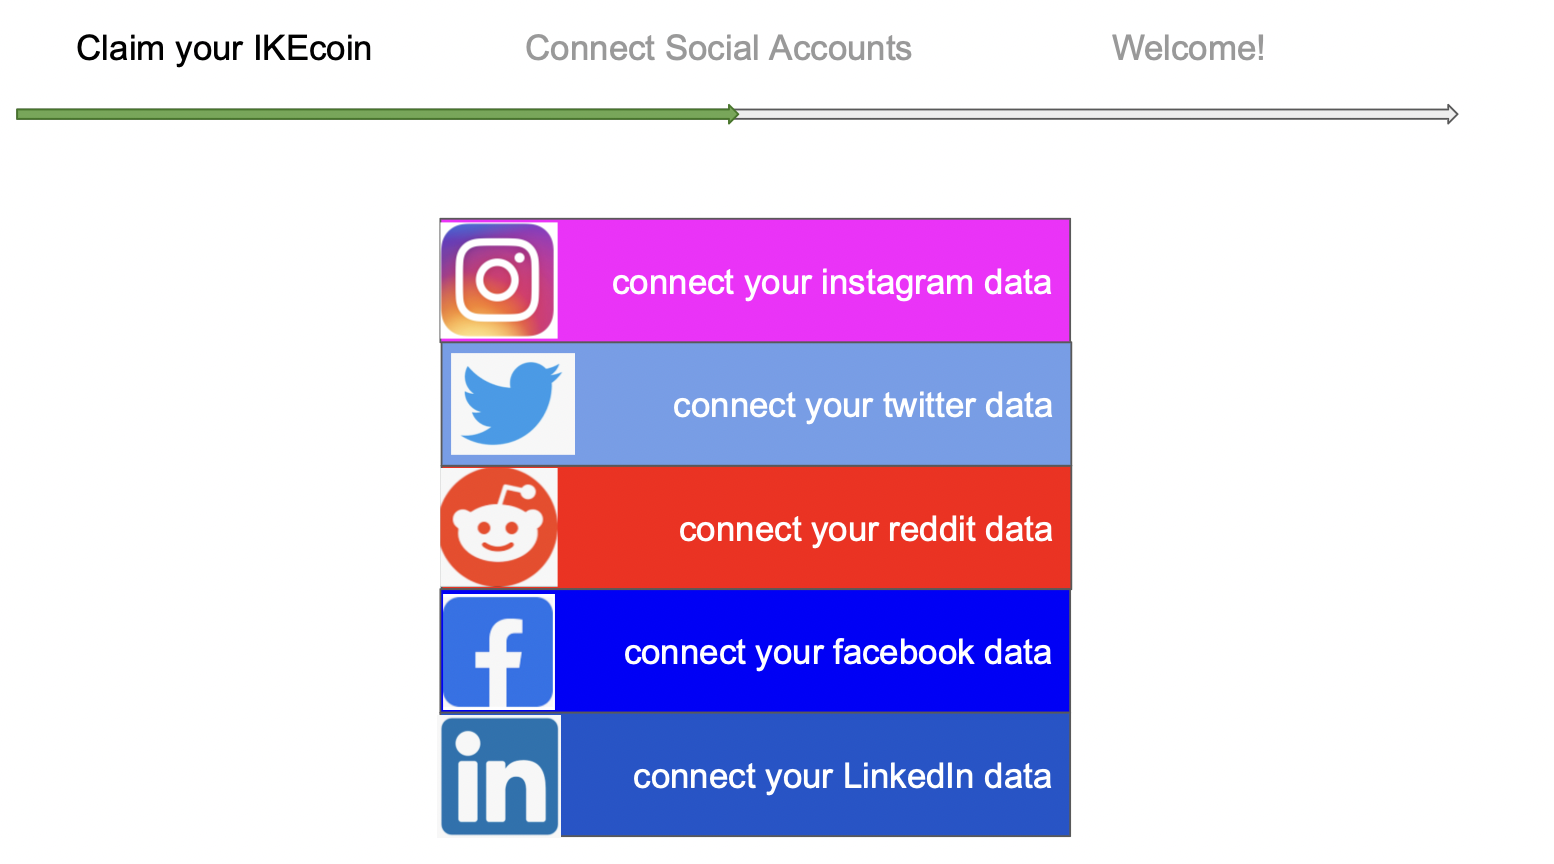
\includegraphics[scale=0.3]{media/AddSocial.jpg}
\centering
\end{figure}
  
\item The value of his data connected to IKEcoin is based on the fair market value for the data, the number of accounts linked, and the size and quality of the data he connected
\begin{figure}[h]
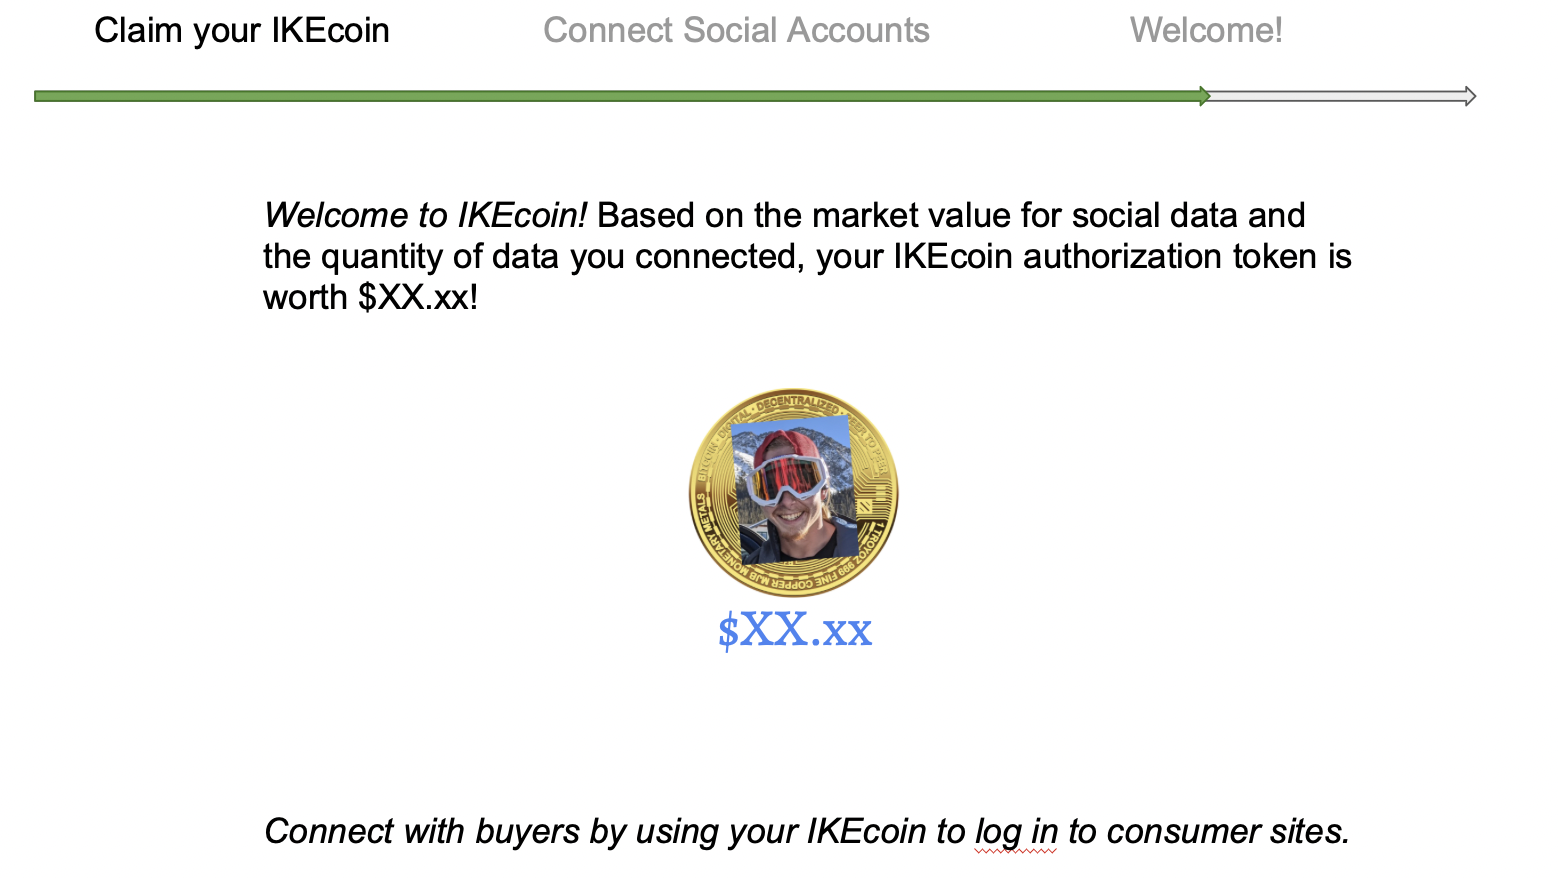
\includegraphics[scale=0.3]{media/Welcome.jpg}
\centering
\end{figure}
   
\item An e-commerce company focused on selling ski equipment has enabled IKEcoin-Auth at login. They have written a clear terms of service agreement detailing how they will use data obtained through IKEcoin-Auth. Isaac accepts this agreement and uses his IKEcoin-Auth to log in to the website 
\begin{figure}[h]
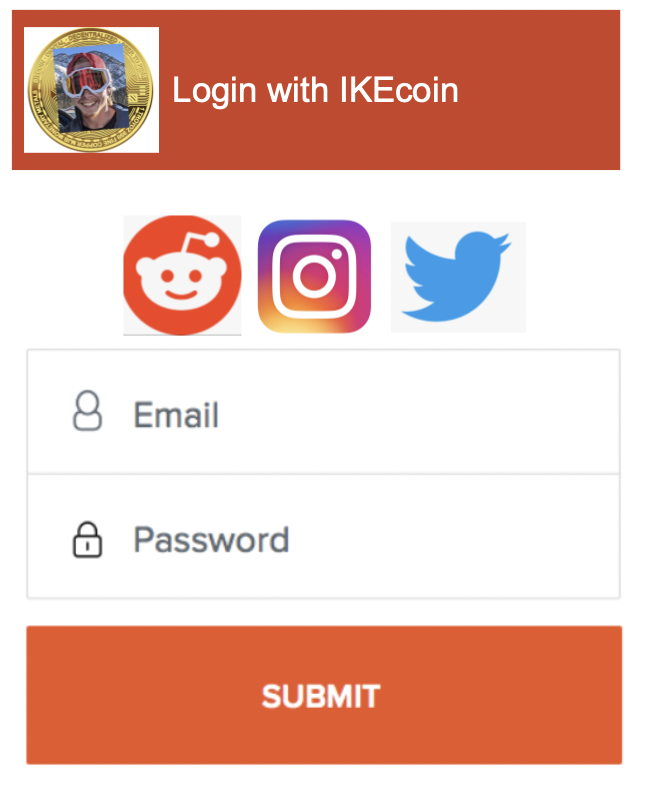
\includegraphics[scale=0.3]{media/IKEcoinLogin.jpg}
\centering
\end{figure}
    
\item The e-commerce site pays Isaac for access to his data  in IKEcoin tokens.
    
\item The e-commerce website uses Isaac's social media data to improve their machine learning algorithm that automatically produces personalized product recommendations 
    
\item Isaac buys the new set of ski boots recommended to him by the machine learning algorithm    
\end{enumerate}

\subsubsection*{Benefit to the User}
\begin{itemize}
  \setlength{\itemsep}{1pt}
  \setlength{\parskip}{0pt}
  \setlength{\parsep}{0pt}
  \item The User directly profit from the sale of their data
  \item The User chooses who they sell their data to
\end{itemize}

\subsubsection*{Benefit to the Customer}
\begin{itemize}
  \setlength{\itemsep}{1pt}
  \setlength{\parskip}{0pt}
  \setlength{\parsep}{0pt}
  \item The customer easily collect large amounts of data on their users to enhance their data-driven projects
  \item The customer obtains direct legal authorization from the user to access and use their data
  \item The data for a single user is already joined across multiple social accounts so the customer can create a experience for their users and easily manage their user's profiles
  \item By allowing users to log in with IKEcoin auth instead of a single social login such as facebook or Instagram, the customer is able to collect data from multiple social media accounts instead of one per user
\end{itemize}

\subsubsection*{Benefit to the Data Curation}
\begin{itemize}
  \setlength{\itemsep}{1pt}
  \setlength{\parskip}{0pt}
  \setlength{\parsep}{0pt}
  \item IKEcoin creates an incentive for Users to create more social median accounts to connect to their IKEcoin
  \item IKEcoin creates an incentive for Users to use each social media platform more as a method to generate more data
\end{itemize}


\section{Roadmap/MVP definition}
The first version of IKEcoin requires the following components of functionality:
\\
\\
\textcolor{yellow}{Website} : the IKEcoin website where users can claim and manage their IKEcoin-Auth and tokens.
\\
\\
\textcolor{yellow}{Software} : a Software Development Kit(SDK )for developers to use to easily integrate IKEcoin-Auth onto their websites.
\\
\\
\textcolor{yellow}{Token} : the decenteralized IKEcoin token. \\


The first version of IKEcoin-Auth will support a limited list of social accounts. We will continue to add new sources of data as we continue to build. The social accounts we will focus on in the MVP are determined based on the quality of data and popularity of the platform. 
\begin{itemize}
  \setlength{\itemsep}{1pt}
  \setlength{\parskip}{0pt}
  \setlength{\parsep}{0pt}
  \item[$-$] Facebook
  \item[$-$] Instagram
  \item[$-$] Linkedin
  \item[$-$] Reddit
  \item[$-$] Twitter
\end{itemize}

\section{Risks}
There are a few main risks identified for this project. Most risks involve the Data Creator's willingness to allow the user sell their own personal data.
\begin{itemize}
  \setlength{\itemsep}{1pt}
  \setlength{\parskip}{0pt}
  \setlength{\parsep}{0pt}
  \item[$\diamond$]  The Data Creators may  choose to shut down user’s access to their own data through the APIs.
  \item[$\diamond$]  The Data Creators may start directly selling the users data to compete with the users in new market.
  \item[$\diamond$]  The Customers may not be willing to pay the users for the data.
\end{itemize}

\end{document}